% Created by tikzDevice version 0.12
% !TEX encoding = UTF-8 Unicode
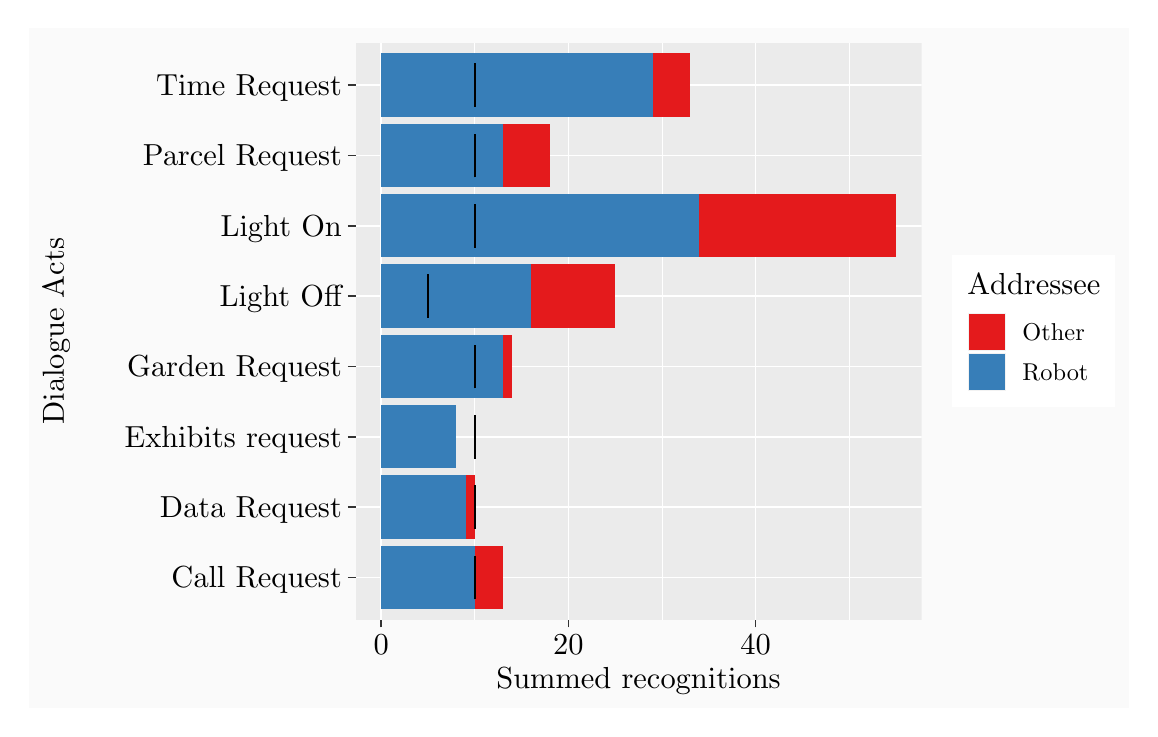
\begin{tikzpicture}[x=1pt,y=1pt]
\definecolor{fillColor}{RGB}{255,255,255}
\path[use as bounding box,fill=fillColor,fill opacity=0.00] (0,0) rectangle (398.34,246.17);
\begin{scope}
\path[clip] (  0.00,  0.00) rectangle (398.34,246.17);
\definecolor{drawColor}{RGB}{255,255,255}
\definecolor{fillColor}{gray}{0.98}

\path[draw=drawColor,line width= 0.6pt,line join=round,line cap=round,fill=fillColor] (  0.00,  0.00) rectangle (398.34,246.17);
\end{scope}
\begin{scope}
\path[clip] (118.48, 32.24) rectangle (323.03,240.67);
\definecolor{fillColor}{gray}{0.92}

\path[fill=fillColor] (118.48, 32.24) rectangle (323.03,240.67);
\definecolor{drawColor}{RGB}{255,255,255}

\path[draw=drawColor,line width= 0.3pt,line join=round] (161.59, 32.24) --
	(161.59,240.67);

\path[draw=drawColor,line width= 0.3pt,line join=round] (229.21, 32.24) --
	(229.21,240.67);

\path[draw=drawColor,line width= 0.3pt,line join=round] (296.83, 32.24) --
	(296.83,240.67);

\path[draw=drawColor,line width= 0.6pt,line join=round] (118.48, 47.49) --
	(323.03, 47.49);

\path[draw=drawColor,line width= 0.6pt,line join=round] (118.48, 72.91) --
	(323.03, 72.91);

\path[draw=drawColor,line width= 0.6pt,line join=round] (118.48, 98.33) --
	(323.03, 98.33);

\path[draw=drawColor,line width= 0.6pt,line join=round] (118.48,123.75) --
	(323.03,123.75);

\path[draw=drawColor,line width= 0.6pt,line join=round] (118.48,149.17) --
	(323.03,149.17);

\path[draw=drawColor,line width= 0.6pt,line join=round] (118.48,174.58) --
	(323.03,174.58);

\path[draw=drawColor,line width= 0.6pt,line join=round] (118.48,200.00) --
	(323.03,200.00);

\path[draw=drawColor,line width= 0.6pt,line join=round] (118.48,225.42) --
	(323.03,225.42);

\path[draw=drawColor,line width= 0.6pt,line join=round] (127.78, 32.24) --
	(127.78,240.67);

\path[draw=drawColor,line width= 0.6pt,line join=round] (195.40, 32.24) --
	(195.40,240.67);

\path[draw=drawColor,line width= 0.6pt,line join=round] (263.02, 32.24) --
	(263.02,240.67);
\definecolor{fillColor}{RGB}{55,126,184}

\path[fill=fillColor] (127.78, 36.05) rectangle (161.59, 58.93);
\definecolor{fillColor}{RGB}{228,26,28}

\path[fill=fillColor] (161.59, 36.05) rectangle (171.73, 58.93);
\definecolor{fillColor}{RGB}{55,126,184}

\path[fill=fillColor] (127.78, 61.47) rectangle (158.21, 84.35);
\definecolor{fillColor}{RGB}{228,26,28}

\path[fill=fillColor] (158.21, 61.47) rectangle (161.59, 84.35);
\definecolor{fillColor}{RGB}{55,126,184}

\path[fill=fillColor] (127.78, 86.89) rectangle (154.82,109.77);

\path[fill=fillColor] (127.78,112.31) rectangle (171.73,135.19);
\definecolor{fillColor}{RGB}{228,26,28}

\path[fill=fillColor] (171.73,112.31) rectangle (175.11,135.19);
\definecolor{fillColor}{RGB}{55,126,184}

\path[fill=fillColor] (127.78,137.73) rectangle (181.87,160.60);
\definecolor{fillColor}{RGB}{228,26,28}

\path[fill=fillColor] (181.87,137.73) rectangle (212.30,160.60);
\definecolor{fillColor}{RGB}{55,126,184}

\path[fill=fillColor] (127.78,163.15) rectangle (242.73,186.02);
\definecolor{fillColor}{RGB}{228,26,28}

\path[fill=fillColor] (242.73,163.15) rectangle (313.73,186.02);
\definecolor{fillColor}{RGB}{55,126,184}

\path[fill=fillColor] (127.78,188.56) rectangle (171.73,211.44);
\definecolor{fillColor}{RGB}{228,26,28}

\path[fill=fillColor] (171.73,188.56) rectangle (188.64,211.44);
\definecolor{fillColor}{RGB}{55,126,184}

\path[fill=fillColor] (127.78,213.98) rectangle (225.83,236.86);
\definecolor{fillColor}{RGB}{228,26,28}

\path[fill=fillColor] (225.83,213.98) rectangle (239.35,236.86);
\definecolor{drawColor}{RGB}{0,0,0}

\path[draw=drawColor,line width= 0.6pt,line join=round] (161.59, 39.64) --
	(161.59, 55.35);

\path[draw=drawColor,line width= 0.6pt,line join=round] (161.59, 47.49) --
	(161.59, 47.49);

\path[draw=drawColor,line width= 0.6pt,line join=round] (161.59, 39.64) --
	(161.59, 55.35);

\path[draw=drawColor,line width= 0.6pt,line join=round] (161.59, 39.64) --
	(161.59, 55.35);

\path[draw=drawColor,line width= 0.6pt,line join=round] (161.59, 47.49) --
	(161.59, 47.49);

\path[draw=drawColor,line width= 0.6pt,line join=round] (161.59, 39.64) --
	(161.59, 55.35);

\path[draw=drawColor,line width= 0.6pt,line join=round] (161.59, 65.06) --
	(161.59, 80.76);

\path[draw=drawColor,line width= 0.6pt,line join=round] (161.59, 72.91) --
	(161.59, 72.91);

\path[draw=drawColor,line width= 0.6pt,line join=round] (161.59, 65.06) --
	(161.59, 80.76);

\path[draw=drawColor,line width= 0.6pt,line join=round] (161.59, 65.06) --
	(161.59, 80.76);

\path[draw=drawColor,line width= 0.6pt,line join=round] (161.59, 72.91) --
	(161.59, 72.91);

\path[draw=drawColor,line width= 0.6pt,line join=round] (161.59, 65.06) --
	(161.59, 80.76);

\path[draw=drawColor,line width= 0.6pt,line join=round] (161.59, 90.47) --
	(161.59,106.18);

\path[draw=drawColor,line width= 0.6pt,line join=round] (161.59, 98.33) --
	(161.59, 98.33);

\path[draw=drawColor,line width= 0.6pt,line join=round] (161.59, 90.47) --
	(161.59,106.18);

\path[draw=drawColor,line width= 0.6pt,line join=round] (161.59,115.89) --
	(161.59,131.60);

\path[draw=drawColor,line width= 0.6pt,line join=round] (161.59,123.75) --
	(161.59,123.75);

\path[draw=drawColor,line width= 0.6pt,line join=round] (161.59,115.89) --
	(161.59,131.60);

\path[draw=drawColor,line width= 0.6pt,line join=round] (161.59,115.89) --
	(161.59,131.60);

\path[draw=drawColor,line width= 0.6pt,line join=round] (161.59,123.75) --
	(161.59,123.75);

\path[draw=drawColor,line width= 0.6pt,line join=round] (161.59,115.89) --
	(161.59,131.60);

\path[draw=drawColor,line width= 0.6pt,line join=round] (144.68,141.31) --
	(144.68,157.02);

\path[draw=drawColor,line width= 0.6pt,line join=round] (144.68,149.17) --
	(144.68,149.17);

\path[draw=drawColor,line width= 0.6pt,line join=round] (144.68,141.31) --
	(144.68,157.02);

\path[draw=drawColor,line width= 0.6pt,line join=round] (144.68,141.31) --
	(144.68,157.02);

\path[draw=drawColor,line width= 0.6pt,line join=round] (144.68,149.17) --
	(144.68,149.17);

\path[draw=drawColor,line width= 0.6pt,line join=round] (144.68,141.31) --
	(144.68,157.02);

\path[draw=drawColor,line width= 0.6pt,line join=round] (161.59,166.73) --
	(161.59,182.44);

\path[draw=drawColor,line width= 0.6pt,line join=round] (161.59,174.58) --
	(161.59,174.58);

\path[draw=drawColor,line width= 0.6pt,line join=round] (161.59,166.73) --
	(161.59,182.44);

\path[draw=drawColor,line width= 0.6pt,line join=round] (161.59,166.73) --
	(161.59,182.44);

\path[draw=drawColor,line width= 0.6pt,line join=round] (161.59,174.58) --
	(161.59,174.58);

\path[draw=drawColor,line width= 0.6pt,line join=round] (161.59,166.73) --
	(161.59,182.44);

\path[draw=drawColor,line width= 0.6pt,line join=round] (161.59,192.15) --
	(161.59,207.86);

\path[draw=drawColor,line width= 0.6pt,line join=round] (161.59,200.00) --
	(161.59,200.00);

\path[draw=drawColor,line width= 0.6pt,line join=round] (161.59,192.15) --
	(161.59,207.86);

\path[draw=drawColor,line width= 0.6pt,line join=round] (161.59,192.15) --
	(161.59,207.86);

\path[draw=drawColor,line width= 0.6pt,line join=round] (161.59,200.00) --
	(161.59,200.00);

\path[draw=drawColor,line width= 0.6pt,line join=round] (161.59,192.15) --
	(161.59,207.86);

\path[draw=drawColor,line width= 0.6pt,line join=round] (161.59,217.57) --
	(161.59,233.28);

\path[draw=drawColor,line width= 0.6pt,line join=round] (161.59,225.42) --
	(161.59,225.42);

\path[draw=drawColor,line width= 0.6pt,line join=round] (161.59,217.57) --
	(161.59,233.28);

\path[draw=drawColor,line width= 0.6pt,line join=round] (161.59,217.57) --
	(161.59,233.28);

\path[draw=drawColor,line width= 0.6pt,line join=round] (161.59,225.42) --
	(161.59,225.42);

\path[draw=drawColor,line width= 0.6pt,line join=round] (161.59,217.57) --
	(161.59,233.28);
\end{scope}
\begin{scope}
\path[clip] (  0.00,  0.00) rectangle (398.34,246.17);
\definecolor{drawColor}{RGB}{0,0,0}

\node[text=drawColor,anchor=base east,inner sep=0pt, outer sep=0pt, scale=  1.10] at (113.53, 43.70) {Call Request};

\node[text=drawColor,anchor=base east,inner sep=0pt, outer sep=0pt, scale=  1.10] at (113.53, 69.12) {Data Request};

\node[text=drawColor,anchor=base east,inner sep=0pt, outer sep=0pt, scale=  1.10] at (113.53, 94.54) {Exhibits request};

\node[text=drawColor,anchor=base east,inner sep=0pt, outer sep=0pt, scale=  1.10] at (113.53,119.96) {Garden Request};

\node[text=drawColor,anchor=base east,inner sep=0pt, outer sep=0pt, scale=  1.10] at (113.53,145.38) {Light Off};

\node[text=drawColor,anchor=base east,inner sep=0pt, outer sep=0pt, scale=  1.10] at (113.53,170.80) {Light On};

\node[text=drawColor,anchor=base east,inner sep=0pt, outer sep=0pt, scale=  1.10] at (113.53,196.22) {Parcel Request};

\node[text=drawColor,anchor=base east,inner sep=0pt, outer sep=0pt, scale=  1.10] at (113.53,221.63) {Time Request};
\end{scope}
\begin{scope}
\path[clip] (  0.00,  0.00) rectangle (398.34,246.17);
\definecolor{drawColor}{gray}{0.20}

\path[draw=drawColor,line width= 0.6pt,line join=round] (115.73, 47.49) --
	(118.48, 47.49);

\path[draw=drawColor,line width= 0.6pt,line join=round] (115.73, 72.91) --
	(118.48, 72.91);

\path[draw=drawColor,line width= 0.6pt,line join=round] (115.73, 98.33) --
	(118.48, 98.33);

\path[draw=drawColor,line width= 0.6pt,line join=round] (115.73,123.75) --
	(118.48,123.75);

\path[draw=drawColor,line width= 0.6pt,line join=round] (115.73,149.17) --
	(118.48,149.17);

\path[draw=drawColor,line width= 0.6pt,line join=round] (115.73,174.58) --
	(118.48,174.58);

\path[draw=drawColor,line width= 0.6pt,line join=round] (115.73,200.00) --
	(118.48,200.00);

\path[draw=drawColor,line width= 0.6pt,line join=round] (115.73,225.42) --
	(118.48,225.42);
\end{scope}
\begin{scope}
\path[clip] (  0.00,  0.00) rectangle (398.34,246.17);
\definecolor{drawColor}{gray}{0.20}

\path[draw=drawColor,line width= 0.6pt,line join=round] (127.78, 29.49) --
	(127.78, 32.24);

\path[draw=drawColor,line width= 0.6pt,line join=round] (195.40, 29.49) --
	(195.40, 32.24);

\path[draw=drawColor,line width= 0.6pt,line join=round] (263.02, 29.49) --
	(263.02, 32.24);
\end{scope}
\begin{scope}
\path[clip] (  0.00,  0.00) rectangle (398.34,246.17);
\definecolor{drawColor}{RGB}{0,0,0}

\node[text=drawColor,anchor=base,inner sep=0pt, outer sep=0pt, scale=  1.10] at (127.78, 19.71) {0};

\node[text=drawColor,anchor=base,inner sep=0pt, outer sep=0pt, scale=  1.10] at (195.40, 19.71) {20};

\node[text=drawColor,anchor=base,inner sep=0pt, outer sep=0pt, scale=  1.10] at (263.02, 19.71) {40};
\end{scope}
\begin{scope}
\path[clip] (  0.00,  0.00) rectangle (398.34,246.17);
\definecolor{drawColor}{RGB}{0,0,0}

\node[text=drawColor,anchor=base,inner sep=0pt, outer sep=0pt, scale=  1.10] at (220.75,  7.44) {Summed recognitions};
\end{scope}
\begin{scope}
\path[clip] (  0.00,  0.00) rectangle (398.34,246.17);
\definecolor{drawColor}{RGB}{0,0,0}

\node[text=drawColor,rotate= 90.00,anchor=base,inner sep=0pt, outer sep=0pt, scale=  1.10] at ( 13.08,136.46) {Dialogue Acts};
\end{scope}
\begin{scope}
\path[clip] (  0.00,  0.00) rectangle (398.34,246.17);
\definecolor{fillColor}{RGB}{255,255,255}

\path[fill=fillColor] (334.03,108.99) rectangle (392.84,163.92);
\end{scope}
\begin{scope}
\path[clip] (  0.00,  0.00) rectangle (398.34,246.17);
\definecolor{drawColor}{RGB}{0,0,0}

\node[text=drawColor,anchor=base west,inner sep=0pt, outer sep=0pt, scale=  1.10] at (339.53,149.87) {Addressee};
\end{scope}
\begin{scope}
\path[clip] (  0.00,  0.00) rectangle (398.34,246.17);
\definecolor{drawColor}{RGB}{255,255,255}
\definecolor{fillColor}{gray}{0.95}

\path[draw=drawColor,line width= 0.6pt,line join=round,line cap=round,fill=fillColor] (339.53,128.95) rectangle (353.98,143.40);
\end{scope}
\begin{scope}
\path[clip] (  0.00,  0.00) rectangle (398.34,246.17);
\definecolor{fillColor}{RGB}{228,26,28}

\path[fill=fillColor] (340.24,129.66) rectangle (353.27,142.69);
\end{scope}
\begin{scope}
\path[clip] (  0.00,  0.00) rectangle (398.34,246.17);
\definecolor{drawColor}{RGB}{255,255,255}
\definecolor{fillColor}{gray}{0.95}

\path[draw=drawColor,line width= 0.6pt,line join=round,line cap=round,fill=fillColor] (339.53,114.49) rectangle (353.98,128.95);
\end{scope}
\begin{scope}
\path[clip] (  0.00,  0.00) rectangle (398.34,246.17);
\definecolor{fillColor}{RGB}{55,126,184}

\path[fill=fillColor] (340.24,115.20) rectangle (353.27,128.24);
\end{scope}
\begin{scope}
\path[clip] (  0.00,  0.00) rectangle (398.34,246.17);
\definecolor{drawColor}{RGB}{0,0,0}

\node[text=drawColor,anchor=base west,inner sep=0pt, outer sep=0pt, scale=  0.88] at (359.48,133.14) {Other};
\end{scope}
\begin{scope}
\path[clip] (  0.00,  0.00) rectangle (398.34,246.17);
\definecolor{drawColor}{RGB}{0,0,0}

\node[text=drawColor,anchor=base west,inner sep=0pt, outer sep=0pt, scale=  0.88] at (359.48,118.69) {Robot};
\end{scope}
\end{tikzpicture}
